% !TEX TS-program = lualatex
% !BIB TS-program = biber
%\documentclass[handout]{beamer}
\documentclass{beamer}
\input{../common/misomva}
%\newcommand{\misoclasstinytitleslide}{Partially based on material by:  Ulrike von Luxburg, \\[-1em] Gary Miller, Doyle \& Schnell, Daniel Spielman}
\newcommand{\misoclasstinytitleslide}{Partially based on material by:   Gary Miller, \\ Mikhail Belkin, Branislav Kveton, \\[-1em] Doyle \& Schnell, Daniel Spielman}
\newcommand{\misoclassdate}{}
\begin{document}
% Topic-specific title slide
\newcommand{\topictitle}{SSL Regularization and Stability}
\newcommand{\topicsubtitle}{Regularized, Soft Harmonic, and Stability Bounds}
\renewcommand{\misoclasstinytitleslide}{Partially based on material by:  Mikhail Belkin, Partha Niyogi, \\[-1em] Olivier Chapelle, Bernhard Sch\"olkopf}

\MakeTopicSlide

\begin{frame}
\frametitle{SSL with Graphs: Regularized Harmonic Functions}

\[
f_i =  p_i^{(+1)} - p_i^{(-1)} \qquad \pause \qquad \implies f_i = \underbrace{|f_i|}_{\rm confidence}\!\!\!\times\ \underbrace{\sgn(f_i)}_{\rm label}
\]

\pause
\questionbox{What if a nasty outlier sneaks in? }
\pause
\rightyellbox{The prediction for the outlier can be hyperconfident :(}
\pause
\questionbox{How to control the confidence of the inference?}
\pause
\begin{center}
Allow the random walk to \emphcol{die}!
\end{center}
\pause
We add a \emphcol{sink} to the graph. \\[0.5em]
\pause
sink = artificial label node with value 0 \\[0.5em]
\pause
We connect it to every other vertex. \\[0.5em]
\pause

\begin{flushright}
\questionbox{What will this do to our predictions?} \\
\pause
\notecol{\tiny depends on the weigh on the edges}
\end{flushright}
\end{frame}

%%%%%%%%%%%%%%%%%%%%%%%%%%%%%%%%%%%%%%%%%%%%%%%%%%%%%%%%%%%%
\begin{frame}
\frametitle{SSL with Graphs: Regularized Harmonic Functions}
\rightquestionbox{How do we represent the sink in $\bL$ explicitly?}
\pause
Formally, to get the harmonic solution on the graph with sink \dots
\pause
\[
\left[\begin{array}{ccc}
\bL_{ll}  +  \gamma_G \bI_{n_l} & \bL_{lu}  & -\gamma_G\bOne_{n_l  \times 1}\\
\bL_{ul} & \bL_{uu} + \gamma_G \bI_{n_u}  & -\gamma_G\bOne_{n_u  \times 1}\\
-\gamma_G \bOne_{1  \times n_l} & -\gamma_G \bOne_{1\times n_u }& n\gamma_G\\
\end{array}\right]
\left[\begin{array}{c}
\bff_{l} \\
\bff_{u} \\
0
\end{array}\right]
=
\left[\begin{array}{c}
\dots\\
\bZero_{u}\\
\dots
\end{array}\right]
\] \pause
\[
 \bL_{ul}\bff_{l} + \left( \bL_{uu} + \gamma_G \bI_{n_u} \right) \bff_{u} = \bZero_{u}
\]
 \pause \dots which is the same if we disregard the last column and row \dots
\[
\left[\begin{array}{cc}
\bL_{ll}  +  \gamma_G \bI_{n_l} & \bL_{lu}  \\
\bL_{ul} & \bL_{uu} + \gamma_G \bI_{n_u}  \\
\end{array}\right]
\left[\begin{array}{c}
\bff_{l} \\
\bff_{u} \\
\end{array}\right]
=
\left[\begin{array}{c}
\dots\\
\bZero_{u}
\end{array}\right]
\]\pause 
\rightyellbox{ \dots and therefore we simply add $\gamma_G$ to the diagonal of $\bL$!}
\end{frame}
%%%%%%%%%%%%%%%%%%%%%%%%%%%%%%%%%%%%%%%%%%%%%%%%%%%%%%%%%%%%
\begin{frame}
\frametitle{SSL with Graphs: Regularized Harmonic Functions}

\questionbox{
How do we compute this \emphcol{regularized} random walk?
}
\pause

\[
 \bff_{u} = \left( \bL_{uu} + \alert{\gamma_g \bI} \right)^{-1}(\bW_{ul}\bff_{l})
\]

\pause

\questionbox{How does $\gamma_g$ influence HS?}

\pause
\begin{center}
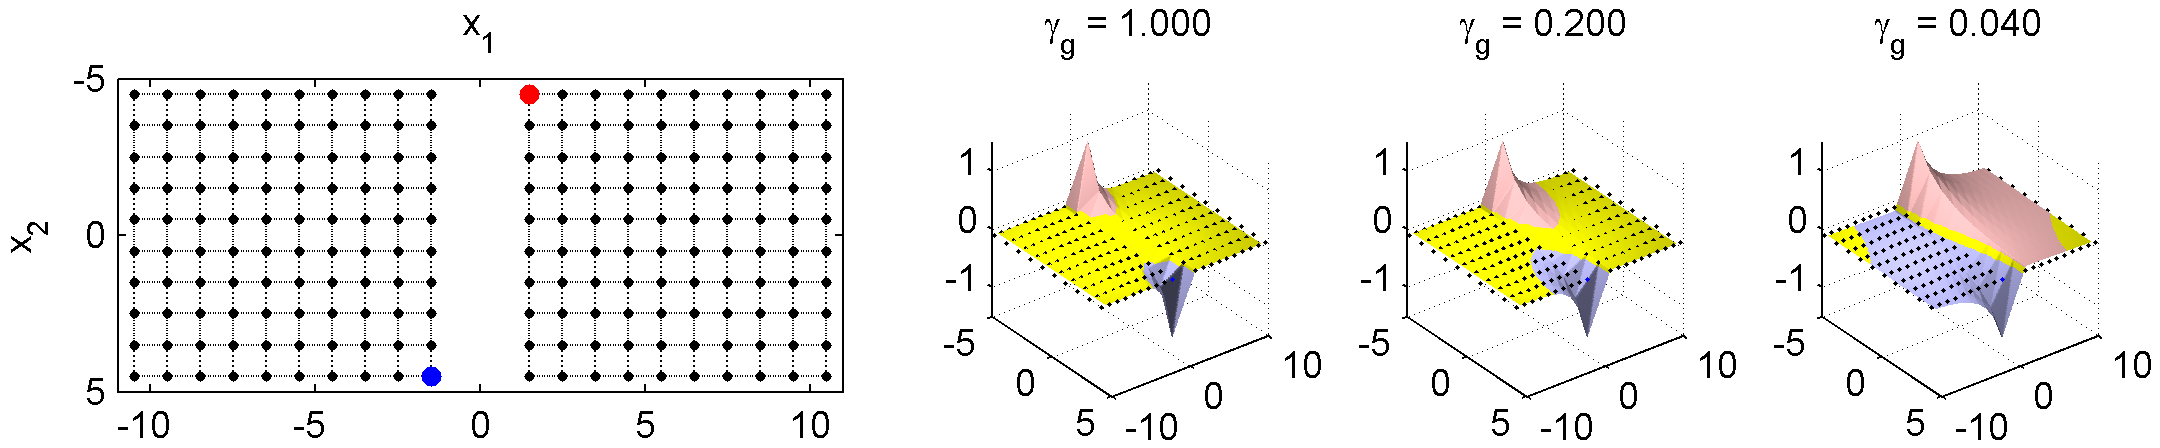
\includegraphics[width=\columnwidth]{../img/HFS}                                                      \end{center}

\pause

\questionbox{What happens to sneaky outliers?}

\end{frame}

%%%%%%%%%%%%%%%%%%%%%%%%%%%%%%%%%%%%%%%%%%%%%%%%%%%%%%%%%%%%

\begin{frame}
\frametitle{SSL with Graphs: Soft Harmonic Functions}

Regularized HS objective with $\bQ = \bL + \gamma_g \bI$: \pause

 \[
   \min_{\bff \in \R^{n_l + n_u} }\mcolA{\infty \sum_{i=1}^{n_l}  \left( f(\bx_i) - y_i \right)^2 }
   + \lambda\mcolB{ \bff\transpose \bQ \bff }
  \]

\pause
\questionbox{
What if we do not really believe that $f(\bx_i) =  y_i$, $\forall i $?}
\pause

\begin{equation*}
  \bff^{\star} = \min_{\bff \in \R^\nodes}  \mcolA{(\bff - \by)\transpose \bC (\bff - \by)} + \mcolB{\bff\transpose \bQ \bff}
\end{equation*}
\pause
$\bC$ is diagonal with 
$C_{ii} =
\begin{cases}
c_l & \mbox{for labeled examples}  \\
c_u & \mbox{otherwise}. \end{cases}
$
\\ \pause
$\by \equiv$  pseudo-targets with 
$y_i =
\begin{cases}
\mbox{true label} & \mbox{for  labeled examples}  \\
0 & \mbox{otherwise}. \end{cases}
$


\end{frame}

%%%%%%%%%%%%%%%%%%%%%%%%%%%%%%%%%%%%%%%%%%%%%%%%%%%%%%%%%%%%
\begin{frame}
\frametitle{SSL with Graphs: Soft Harmonic Functions}

\begin{equation*}
  \bff^{\star} = \min_{\bff \in \R^n}  \mcolA{(\bff - \by)\transpose \bC (\bff - \by)} + \mcolB{\bff\transpose \bQ \bff}
\end{equation*}

Closed form \emphcol{soft harmonic solution}:  
\pause
\begin{equation*}
\bff^\star  = (\bC^{-1}\bQ+ \bI)^{-1}\by
\end{equation*}
\begin{center}
\pause
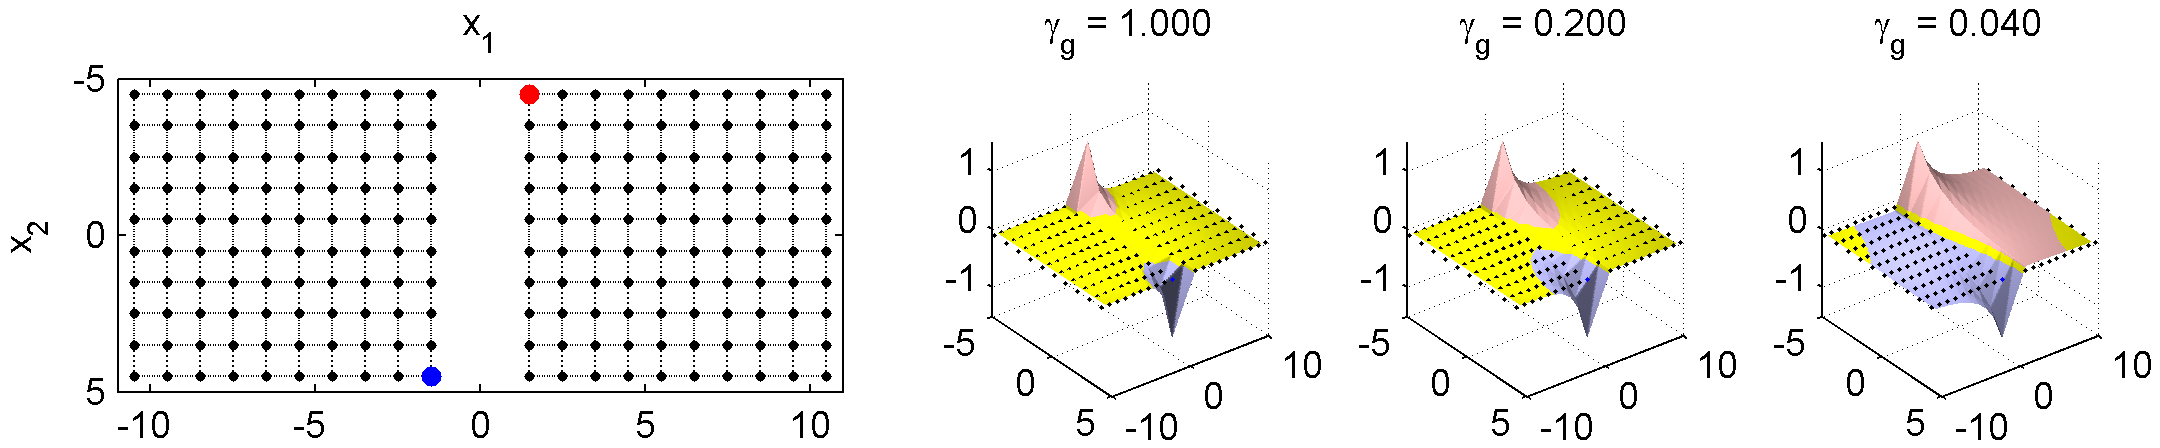
\includegraphics[width=\columnwidth]{../img/HFS}                                                      \end{center}
\pause
\begin{flushright}
\questionbox{What are the differences between hard and soft?}
\pause
\yellbox{Not much different in practice.}  
\pause
\yellbox{Provable generalization guarantees for the soft one.}\end{flushright}
\end{frame}

%%%%%%%%%%%%%%%%%%%%%%%%%%%%%%%%%%%%%%%%%%%%%%%%%%%%%%%%%%%%
\begin{frame}
\frametitle{SSL with Graphs: Stability Bounds}
\begin{align*}
  \bff^\star = \min_{\bff \in \realset^\nodes} \
  (\bff - \by)\transpose \bC (\bff - \by) +
  \bff\transpose \bQ \bff
\end{align*}
\pause
Think about \emphcol{stability} of this solution. \\
\pause
Consider two datasets differing in exactly one \textit{labeled} point.
\pause
$\cC_1 = \bC_1^{-1}\bQ + \bI$
and 
$\cC_2 = \bC_2^{-1}\bQ + \bI$\\
\pause
\rightquestionbox{What is the maximal difference in the solutions?}
\pause
\begin{align*}
\action<+->{\bff_2^\star - \bff_1^\star}
 \action<+->{& = \cC_2^{-1}\by_2 - \cC_1^{-1}\by_1 } \\
 \action<+->{& = \cC_2^{-1}(\by_2 - \by_1) - \left(\cC_1^{-1}-\cC_2^{-1} \right)\by_1 } \\
 \action<+->{& = \cC_2^{-1}(\by_2 - \by_1) - \left( \cC_1^{-1} \left[ \left(\bC_1^{-1}-\bC_2^{-1} \right)\bQ\right]\cC_2^{-1} \right)\by_1 }
\end{align*}
\pause
\vskip -1em
\mbox{\notecol{\tiny 
Note that
$\bv \in \realset^{\nodes \times 1}$, $\lambda_m (A)\|\bv\|_2 \leq \| A\bv \|_2 \leq \lambda_M (A) \|\bv\|_2$} }
\pause
\[
    \normtwo{\bff_2^\star - \bff_1^\star} \pause
    \leq  \frac{\normtwo{\by_2 - \by_1}}{\lambda_m(\cC_2)}
    \pause + \frac{\lambda_M(\bQ) \pause \normtwo{\bC_1^{-1}-\bC_2^{-1}
    } \pause \cdot \normtwo{\by_1}}{\pause\lambda_m(\cC_2)\lambda_m(\cC_1)}
    \]

    \end{frame}
    %%%%%%%%%%%%%%%%%%%%%%%%%%%%%%%%%%%%%%%%%%%%%%%%%%%%%%%%%%%%
    \begin{frame}
    \frametitle{SSL with Graphs: Stability Bounds}
    \begin{align*}
      \bff^\star = \min_{\bff \in \realset^\nodes} \
      (\bff - \by)\transpose \bC (\bff - \by) +
  \bff\transpose \bQ \bff
\end{align*}

\[
\normtwo{\bff_2^\star - \bff_1^\star} 
\leq  \frac{\normtwo{\by_2 - \by_1}}{\lambda_m(\cC_2)}
 + \frac{\lambda_M(\bQ)  \normtwo{\bC_1^{-1}-\bC_2^{-1}
}  \cdot \normtwo{\by_1}}{\lambda_m(\cC_2)\lambda_m(\cC_1)}
\]

\pause
Using $\lambda_m(\cC) \geq \frac{\lambda_m(\bQ)}{\lambda_M(\bC)} + 1$
\pause
\[
\normtwo{\bff_2^\star - \bff_1^\star} 
\leq  \frac{\normtwo{\by_2 - \by_1}}{\frac{\lambda_m(\bQ)}{\lambda_M(\bC_1)} + 1}
 + \frac{\lambda_M(\bQ) \normtwo{\bC_1^{-1}-\bC_2^{-1}
}  \cdot \normtwo{\by_1}}{\left( \frac{\lambda_m(\bQ)}{\lambda_M(\bC_2)} + 1 \right)
\left(  \frac{\lambda_m(\bQ)}{\lambda_M(\bC_1)} + 1  \right)}
\]


\end{frame}
%%%%%%%%%%%%%%%%%%%%%%%%%%%%%%%%%%%%%%%%%%%%%%%%%%%%%%%%%%%%
\begin{frame}
\frametitle{SSL with Graphs: Stability Bounds}
\[
 \norminf{\bff_2^\star - \bff_1^\star} 
\leq  \alert{\beta} \leq \frac{\normtwo{\by_2 - \by_1}}{\frac{\lambda_m(\bQ)}{\lambda_M(\bC_1)} + 1}
 + \frac{\lambda_M(\bQ) \normtwo{\bC_1^{-1}-\bC_2^{-1}
}  \cdot \normtwo{\by_1}}{\left( \frac{\lambda_m(\bQ)}{\lambda_M(\bC_2)} + 1 \right)
\left(  \frac{\lambda_m(\bQ)}{\lambda_M(\bC_1)} + 1  \right)}
\]

\pause
Now, let us plug in the values for our problem.
\pause
\moveb
Take $c_l = 1$ \pause and $c_l > c_u$. \pause
We have $\abs{y_i} \leq 1$ \pause and $\abs{f_i^\star} \leq 1$. \pause
\begin{align*}
  \beta \leq 2 \left[\frac{\sqrt{2}}{\lambda_m(\bQ) + 1} +
  \sqrt{2 n_l} \frac{1 - c_u}{c_u}
  \frac{\lambda_M(\bQ)}{(\lambda_m(\bQ) + 1)^2}\right]
\end{align*}
\pause 
$\bQ$ is reg.\@ $\bL$:
$\lambda_m(\bQ) = \lambda_m(\bL) + \gamma_g$
\pause and 
$\lambda_M(\bQ) = \lambda_M(\bL) + \gamma_g$
\pause
\begin{align*}  
  \beta \ \leq & \ \
  2 \left[\frac{\sqrt{2}}{\gamma_g + 1} +
  \sqrt{2 n_l} \frac{1 - c_u}{c_u}
  \frac{\lambda_M(\bL) + \gamma_g}{\gamma_g^2 + 1}\right]
\end{align*}
\pause
\rightyellbox{This algorithm is $\beta$-stable!}

\end{frame}

%%%%%%%%%%%%%%%%%%%%%%%%%%%%%%%%%%%%%%%%%%%%%%%%%%%%%%%%%%%%
\begin{frame}
\frametitle{SSL with Graphs: Regularized Harmonic Functions}

\textbf{Larger implications of random walks} \\[0.5em]

random walk relates to \emphcol{commute distance}
\pause 
which should satisfy \\[0.5em]

\begin{block}{}
($\star$) Vertices in the \textbf{same} cluster of the graph have a \textbf{small} commute
distance, whereas two vertices in \textbf{different} clusters of the graph have a \textbf{large}
commute distance.
\vspace{0.5em}
\end{block}
\pause 
\questionbox{Do we have this property for HS?}
\pause 
\questionbox{What if $\nodes\to\infty$?} \\[0.5em]
\pause 

{\small Luxburg/Radl/Hein: \textit{Getting \alert{lost} in space: Large sample analysis of the
commute distance}}
{\scriptsize 
\url{http://www.informatik.uni-hamburg.de/ML/contents/people/luxburg/publications/LuxburgRadlHein2010_PaperAndSupplement.pdf}
}
\\[0.5em]
\pause
\questionbox{Solutions?}
\pause 
1) $\gamma_g$
\pause 
2) amplified commute distance
\pause 
3) $\bL^p$
\pause  $\dots$ \\[0.5em]
\pause

The goal of these solutions: \pause
\textbf{make them remember!}

\end{frame}
%%%%%%%%%%%%%%%%%%%%%

\begin{frame}
\frametitle{SSL with Graphs: Out of sample extension}

Both \textbf{MinCut} and \textbf{HFS} only inferred the labels
on unlabeled data. \\[1em]
They are \pause \emphcol{transductive}.
\\[1em] \pause
\questionbox{What if a new point $\bx_{n_l+n_u + 1}$ arrives?}
\pause
\grcol{\tiny also called out-of-sample extension} \\[1em]
\pause
\textbf{Option 1)} Add it to the graph and recompute HFS. \\[1em]
\pause
\textbf{Option 2)} Make the algorithms \emphcol{inductive}! \\[1em]
\pause
Allow to be defined everywhere: $f: \cX \mapsto \R$ \\
\pause
Allow $f(\bx_i) \ne y_i$. \pause \questionbox{Why?} \pause To deal with noise.\\[1em]
\pause
Solution: \emphcol{Manifold Regularization}
\end{frame}


\MakeLastSlide
\end{document}
